\documentclass{article}
\documentclass{article}
\usepackage[utf8]{inputenc}
\usepackage{fullpage}
\usepackage{amsmath, mathtools}
\usepackage{amsfonts}
\usepackage{amssymb}
\usepackage{graphicx}
\usepackage{colortbl}
\usepackage{xr}
\usepackage{hyperref}
\usepackage{longtable}
\usepackage{xfrac}
\usepackage{tabularx}
\usepackage{float}
\usepackage{siunitx}
\usepackage{booktabs}
\usepackage{caption}
\usepackage{pdflscape}
\usepackage{afterpage}
\usepackage{seqsplit}
\usepackage{underscore}
\usepackage{lscape}
\usepackage[english]{babel}
\usepackage[T1]{fontenc}
\usepackage{booktabs}
\usepackage{tabularx}
\usepackage{hyperref}

\hypersetup{
    colorlinks=true,       % false: boxed links; true: colored links
    linkcolor=red,          % color of internal links (change box color with linkbordercolor)
    citecolor=green,        % color of links to bibliography
    filecolor=magenta,      % color of file links
    urlcolor=cyan           % color of external links
}

%% Comments

\usepackage{color}

\newif\ifcomments\commentstrue %displays comments
%\newif\ifcomments\commentsfalse %so that comments do not display

\ifcomments
\newcommand{\authornote}[3]{\textcolor{#1}{[#3 ---#2]}}
\newcommand{\todo}[1]{\textcolor{red}{[TODO: #1]}}
\else
\newcommand{\authornote}[3]{}
\newcommand{\todo}[1]{}
\fi

\newcommand{\wss}[1]{\authornote{blue}{SS}{#1}} 
\newcommand{\plt}[1]{\authornote{magenta}{TPLT}{#1}} %For explanation of the template
\newcommand{\an}[1]{\authornote{cyan}{Author}{#1}}

%% Common Parts

\newcommand{\progname}{Mechatronics Engineering} % PUT YOUR PROGRAM NAME HERE
\newcommand{\authname}{Team \# 34, ParkingLotHawk
\\ Fady Zekry Hanna, zekryhf
\\ Winnie Trandinh, trandint
\\ Muhammad Ali, alim102
\\ Muhammad Khan, khanm120} % AUTHOR NAMES                  

\usepackage{hyperref}
    \hypersetup{colorlinks=true, linkcolor=blue, citecolor=blue, filecolor=blue,
                urlcolor=blue, unicode=false}
    \urlstyle{same}
                                


\title{Hazard Analysis\\\progname}

\author{\authname}

\date{}

\begin{document}

\maketitle
\thispagestyle{empty}

~\newpage

\pagenumbering{roman}

\begin{table}[hp]
\caption{Revision History} \label{TblRevisionHistory}
\begin{tabularx}{\textwidth}{llX}
\toprule
\textbf{Date} & \textbf{Developer(s)} & \textbf{Change}\\
\midrule
Date1 & Name(s) & Description of changes\\
Date2 & Name(s) & Description of changes\\
... & ... & ...\\
\bottomrule
\end{tabularx}
\end{table}

~\newpage

\tableofcontents

~\newpage

\pagenumbering{arabic}

\wss{You are free to modify this template.}
%%%%%%%% --------------------------------------------DOCUMENT START --------------------------------------------%%%%%%%%




%%%%%%%% --------------------------------------------INTRODUCTION --------------------------------------------%%%%%%%%



\section{Introduction}

\wss{You can include your definition of what a hazard is here.}




%%%%%%%% --------------------------------------------Scope and Purpose of Hazard Analysis --------------------------------------------%%%%%%%%
\section{Scope and Purpose of Hazard Analysis}

%%%%%%%% --------------------------------------------Scope and Purpose of Hazard Analysis --------------------------------------------%%%%%%%%
\section{Scope and Purpose of Hazard Analysis}

The purpose of the Hazard Analysis is to find, understand and finalize resolutions to the various hazards that may occur.

The product, ParkingLotHawk, is an Autonomous Aerial Drone used to gather live images and data within the confines of any given outdoor parking lot. The data in drone records the situation of each parking space periodically, and the information would be sent to the user staying on the property in a timely manner. The user of such a product is the Parking Lot Operator (called Operator for short), who communicates with the Aerial Drone using an application running on their PC.

The document starts by breaking the system into components, followed by identifying hazards for each component using the Failure Modes and Effects Analysis (FMEA) method, and then finally generating new safety requirements to resolve the various hazards. This method will help minimize any unsafe behavior in the system by finding any possible causes of the said failure and determining the proper response for it.

%%%%%%%% --------------------------------------------System Boundaries and Components --------------------------------------------%%%%%%%%
\section{System Boundaries and Components}
The systems referenced in this document for conducting ParkingLotHawk’s hazard analysis are:

\begin{table}[!h]
\begin{center}
\caption {System Components Table} 
\label{tab:SystemComp}
\begin{tabular}{ | m{4 cm} | m{12 cm} | } 
\hline
Components & Description \\
\hline
Flight Operations & This component consists of the flight controller and firmware that identifies different measurements during use. The sensors and systems in use are the Inertial Measurement Unit (IMU), the Global Positioning System (GPS), compass for direction and barometer for atmospheric pressure identifying altitude.\\
\hline
Vision Perception & The Vision Perception component has a camera and an algorithm for detecting parking spots.\\
\hline
Aerial Drone Application & This component consists of finite state machines and Application Programming Interfaces (APIs) that were specified in the Software Requirements Specification.\\
\hline
Path Planner & This software component creates an internal map for autonomous exploration.\\
\hline
Thrust & The Thrust Component is what allows the drone to elevate and navigate aerially. The component consists of motors, propellers and  the Electronic Speed Controllers (ESCs).\\
\hline
Chassis Frame & The CAD designed Chassis Frame will hold all the physical pieces of the project together.\\
\hline
Power Modules & The Power Modules will power components within the drone such as the flight controller and motors. The component consists of a battery, charging equipment, and switches and wires.\\
\hline
Operator's PC Application & This component is what the operator interfaces with to get the product up and running.\\
\hline

\end{tabular}
\end{center}
\end{table}


Below is  Diagram \ref{fig:SystemCompDiagram} visualizing all the system components within the project. 


\begin{figure}[!h]
    \centering
    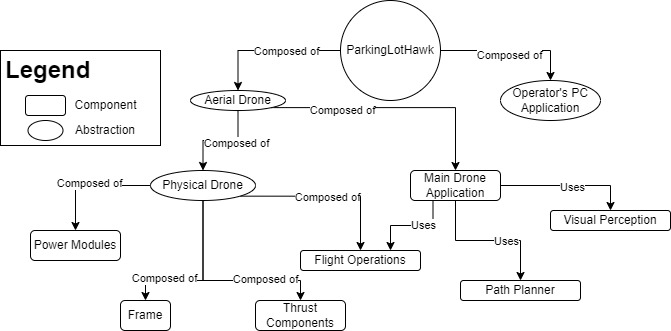
\includegraphics[width=1\textwidth]{HA/System Components.jpg}
    \caption{Systems Components Diagram}
    \label{fig:SystemCompDiagram}
\end{figure}



\newpage
%%%%%%%% --------------------------------------------Critical Assumptions --------------------------------------------%%%%%%%%


\section{Critical Assumptions}
There are several assumptions that help to solve and sometimes even eliminate hazards all together. Firstly, it is assumed that the Parking Lot Operator utilizing the Drone has completely read the User Manual, and that they utilize the drone in the way specified by the user Manual. For example, if the User Manual specifies weather conditions under which the drone should not be flown, it is assumed that the user then does not fly the drone in these inclement weather conditions. Secondly, it is assumed that the operator uses the drone solely for parking lot investigation, not for activities such as recreation, spying, etc.  


%%%%%%%% --------------------------------------------Failure Mode and Effect Analysis --------------------------------------------%%%%%%%%
\section{Failure Mode and Effect Analysis}


\begin{landscape}
\begin{table}[!h]
\begin{center}
\caption {FMEA Table related to Flight Operation Components.} 
\label{tab:FMEA_Flight}
\begin{tabular}{ | m{1.2 cm} | m{3cm} | m{3cm} | m{1cm} | m{2.5 cm} | m{0.7cm} | m{0.6cm} | m{0.6cm} | m{3.5cm}| m{0.5cm} | m{0.5cm} | } 
\hline
 Design Component & Failure Mode & Effect of Failure & \seqsplit{Severity} & Causes of Failure & \seqsplit{Occurrence} & \seqsplit{Detection} & RPN & Recommended Action & SR & Ref \\
\hline
Flight Operation & IMU gives inaccurate readings. & The Drone is unable to determine angular orientation, which makes flight motion and stabilization difficult. & - &  IMU damaged during flight, magnetic interference. -  & - & - & - &  Implement Flight Controller with secondary IMU, providing diversity and redundancy. & \ref{SR_004} & - \\
\hline
Flight Operation & Compass gives inaccurate readings. & Drone has difficulty in determining heading in space. & - & Compass damaged during flight, magnetic interference. -  & - & - & - &  Implement Flight Controller with secondary compass, providing diversity and redundancy. & \ref{SR_004} & - \\
\hline
Flight Operation & Barometer gives an inaccurate reading. & Flight controller unable to determine altitude, creates difficulty in landing. & - & Barometer damaged during flight, UV/motor backwash interference.  & -  & - & - &   Add an ultrasonic sensor at the bottom of the drone. A sensor in such a configuration provides a secondary height estimate. Although this only works for a short range (0-2m) it is sufficient for landing. & \ref{SR_005} & -  \\
\hline
Flight Operation & Firmware unable to make the drone hover in place. Hovering was specified as stabilizing and staying within some tolerance of a location in space for a sufficiently long time. & Drone will not be able to fly to locations or follow paths well. Drone being unable to hover means that the camera will see blurry and shaky images. & - & Flight Controller internal malfunction, inclement weather (such as high winds).  & -  & - & - &   Mention maximum wind requirement in User Manual. Report malfunction to operator and enter Malfunction state. & \ref{SR_006}, \ref{SR_007} & -  \\
\hline
Flight Operation & GPS Connection is lost or weak. & The drone will have a less accurate estimate of position, and thus won't be able to perform autonomous missions or move to a specific GPS locations.  & - & GPS damaged during flight, magnetic interference. -  & - & - & - &  Implement an alternative localization method via the camera or other range finder sensor, such as SLAM or optical flow.  & \ref{SR_008} & - \\
\hline
\end{tabular}
\end{center}
\end{table}
\end{landscape}

\begin{landscape}
\begin{table}[!h]
\begin{center}
\caption {FMEA Table related to Visual Perception.} 
\label{tab:FMEA_Vision}
\begin{tabular}{ | m{1.2 cm} | m{3cm} | m{3cm} | m{1cm} | m{2.5 cm} | m{0.7cm} | m{0.6cm} | m{0.6cm} | m{3.5cm}| m{0.5cm} | m{0.5cm} | }  
\hline
Design Component & Failure Mode & Effect of Failure & Severity & Causes of Failure & \seqsplit{Occurrence} & \seqsplit{Detection} & RPN & Recommended Action & SR & Ref \\
\hline
Visual Perception & Camera gives poor quality images or no image at all. & The primary functionality of showing the operator the parking lot cannot be accomplished. The camera cannot detect the boundaries of the parking lot, causing the drone to be unable to perform autonomous tasks. & - & Camera lens is foggy or has other obstructions, the camera is damaged during flight. -  & - & - & - &  Operator will detect the low image resolution themselves while they watch live video. Operators may choose to wait, may choose to land the drone, clean the lens, restart the drone, and/or reconfigure it to fly closer to the ground.  & \ref{SR_001} & - \\
\hline
Visual Perception & Drone fails to detect the parking lot. & Drone is unable to implement autonomous states, and can only implement manual movement commands.  & - & Perception algorithm performs poorly due to weather conditions or the uniqueness of the parking lot. -  & - & - & - &  Operator should notice from the live camera images that the drone is consistently failing to correctly segment the parking lot, and thus the drone is only useful for true manual movement.  & \ref{SR_006}, \ref{SR_009} & - \\
\hline
- & Drone fails to detect the boundaries of the parking lot. & Drone is unable to implement autonomous states, and can only implement manual movement commands. During an autonomous state, the drone may exit the parking lot and not have noticed.  & - & Perception algorithm performs poorly due to weather conditions or the uniqueness of the parking lot.  & - & - & - &  Operator should notice from the live camera images that the drone is consistently failing to correctly segment the parking lot, and thus the drone is only useful for true manual movement.  & \ref{SR_006}, \ref{SR_009} & - \\
\hline
\end{tabular}
\end{center}
\end{table}
\end{landscape}

\begin{landscape}
\begin{table}[!h]
\begin{center}
\caption {FMEA Table related to the Thrust Components and the Frame.} 
\label{tab:FMEA_Thrust}
\begin{tabular}{ | m{1.2 cm} | m{3cm} | m{3cm} | m{1cm} | m{2.5 cm} | m{0.7cm} | m{0.6cm} | m{0.6cm} | m{3.5cm}| m{0.5cm} | m{0.5cm} | }  
\hline
Design Component & Failure Mode & Effect of Failure & Severity & Causes of Failure & \seqsplit{Occurrence} & \seqsplit{Detection} & RPN & Recommended Action & SR & Ref \\
\hline
Thrust Components, Frame & An arm of the copter is unable to perform, detected by the flight controller or noticed by the operator. & The drone has fewer active propellers than it was tuned, trained, and designed for.  This will cause difficulty in flight and stabilization. & - & The given arm has a damaged propeller, damaged motor, broken electrical disconnection between motor and ESC, or mechanical disconnection between propeller and motor. Also if one of the arms on the frame cracks to the extent of not being able to provide a rigid frame. -  & - & - & - &  Although flight will be hindered, the firmware has the capabilities to still fly the drone under most conditions. The Drone shall enter the malfunction state, trying to land at its original location. The operator, being from a non-technical background, will need to send the drone for repair. In the user manual, it should be specified that the Operator should is required to inspect the drone for damage prior to flight.  & \ref{SR_002}, \ref{SR_007} & - \\
\hline
\end{tabular}
\end{center}
\end{table}
\end{landscape}

\begin{landscape}
\begin{table}[!h]
\begin{center}
\caption {FMEA Table related to the Frame.} 
\label{tab:FMEA_Frame}
\begin{tabular}{ | m{1.2 cm} | m{3cm} | m{3cm} | m{1cm} | m{2.5 cm} | m{0.7cm} | m{0.6cm} | m{0.6cm} | m{3.5cm}| m{0.5cm} | m{0.5cm} | }  
\hline
Design Component & Failure Mode & Effect of Failure & Severity & Causes of Failure & \seqsplit{Occurrence} & \seqsplit{Detection} & RPN & Recommended Action & SR & Ref \\
\hline
Frame & Center of frame cracked, seen by Operator. &  Drone will have difficulty in flight. Parts of Drone may fall out if crack is large enough.  & - & Center of frame damaged during flight. & - & - & - &  Enclose the central base of the drone, so that components do not fall out. In user manual, specify that the Operator is required to inspect drone for damage prior to flight. If the operator sees crack during flight, they should send the Drone into the malfunction state. & \ref{SR_001}, \ref{SR_002}  & - \\
\hline
Frame & Drone is very hot. &  Operator may be hurt if they touch the hot parts. Drone components may also be damaged after prolonged heat exposure. & - & Overheating components. & - & - & - &  Add heat sinks on electrical components, and specify the correct way to hold the drone in user manual. Also specify how long  the operator must wait and let the drone cool down before making any contact with it. & \ref{SR_010} & - \\
\hline
\end{tabular}
\end{center}
\end{table}
\end{landscape}

\begin{landscape}
\begin{table}[!h]
\begin{center}
\caption {FMEA Table related to the Power Modules.} 
\label{tab:FMEA_Power}
\begin{tabular}{ | m{1.2 cm} | m{3cm} | m{3cm} | m{1cm} | m{2.5 cm} | m{0.7cm} | m{0.6cm} | m{0.6cm} | m{3.5cm}| m{0.5cm} | m{0.5cm} | }  
\hline
Design Component & Failure Mode & Effect of Failure & Severity & Causes of Failure & \seqsplit{Occurrence} & \seqsplit{Detection} & RPN & Recommended Action & SR & Ref \\
\hline
Power Modules & Low Battery. &  Drone will be unable to fly for a long duration of time.  & - & Drone has been flying for a long duration. Recharge is not complete.  & - & - & - &  Once the Drone detects less than 3 minutes of battery remaining, it shall automatically land the drone at it's original launch location and inform the operator. & \ref{SR_003} & - \\
\hline
Power Modules & Battery capacity low. &  Drone will be unable to fly long enough to complete its functions. & - & Drone's battery life has deteriorated over time.  & - & - & - &  Drone should prevent flight if the battery capacity is less than 3 minutes, the Drone should convey to operator it cannot fly and reason why. The Operator will need to purchase a new battery.  & \ref{SR_003} & - \\
\hline
Power Modules & Wire connections become loose. &  Electrical components  and system will not function correctly. & - & Wires come loose after extended time of flight or upon damage. & - & - & - &  Solder all electrical wires and attach heat shrinks or crimps to wire-to-wire connections.  & - & - \\
\hline
\end{tabular}
\end{center}
\end{table}
\end{landscape}

\begin{landscape}
\begin{table}[!h]
\begin{center}
\caption {FMEA Table related to the Operator's PC Application.} 
\label{tab:FMEA_OpApp}
\begin{tabular}{ | m{1.2 cm} | m{3cm} | m{3cm} | m{1cm} | m{2.5 cm} | m{0.7cm} | m{0.6cm} | m{0.6cm} | m{3.5cm}| m{0.5cm} | m{0.5cm} | }  
\hline
Design Component & Failure Mode & Effect of Failure & Severity & Causes of Failure & \seqsplit{Occurrence} & \seqsplit{Detection} & RPN & Recommended Action & SR & Ref \\
\hline
\seqsplit{Operator's} PC Application & Malicious user hacks into Operator's PC Application via login system. &  Malicious user will be able to inspect the parking lot.  & - & Too simple of a login password or password leaked out.  & - & - & - &  Require that the passwords be sufficiently complicated: at least one upper case, one lower case, one number and one special character. Also denote in the user manual that the password should be kept a secret from external parties. & - & - \\
\hline
\end{tabular}
\end{center}
\end{table}
\end{landscape}

\begin{landscape}
\begin{table}[!h]
\begin{center}
\caption {FMEA Table related to the Operator's PC Application.} 
\label{tab:FMEA_OpApp}
\begin{tabular}{ | m{1.2 cm} | m{3cm} | m{3cm} | m{1cm} | m{2.5 cm} | m{0.7cm} | m{0.6cm} | m{0.6cm} | m{3.5cm}| m{0.5cm} | m{0.5cm} | }  
\hline
Design Component & Failure Mode & Effect of Failure & Severity & Causes of Failure & \seqsplit{Occurrence} & \seqsplit{Detection} & RPN & Recommended Action & SR & Ref \\
\hline
Path Planner (also called Autonomous Explore) & Internal explore strategy malfunctions. The Operator notices the drone is not exploring the parking lot correctly. &  Drone may keep exploring the same area thus wasting time, or the drone may exit the parking lot.  & - & Due to the path planning algorithm not performing accurately/correctly.  & - & - & - &  It is upon the Operator to notice the inaccuracy of the path planning feature during the Autonomous Explore State. At which point the operator should utilize other more accurate features instead (such as Manual Explore). & - & - \\
\hline
\end{tabular}
\end{center}
\end{table}
\end{landscape}

\begin{landscape}
\begin{table}[!h]
\begin{center}
\caption {FMEA Table related to the Operator's PC Application and the Main Drone Application.} 
\label{tab:FMEA_MainApp_OpApp}
\begin{tabular}{ | m{1.2 cm} | m{3cm} | m{3cm} | m{1cm} | m{2.5 cm} | m{0.7cm} | m{0.6cm} | m{0.6cm} | m{3.5cm}| m{0.5cm} | m{0.5cm} | }  
\hline
Design Component & Failure Mode & Effect of Failure & Severity & Causes of Failure & \seqsplit{Occurrence} & \seqsplit{Detection} & RPN & Recommended Action & SR & Ref \\
\hline
\seqsplit{Operator's} PC Application, Main Drone Application & Drone loses connection to Operator's PC Application, or connection has deteriorated. For example, the connection has been lost for sufficiently long, the connection is very slow, weak and/or delayed. &  Drone is unable to communicate to the operator. The drone is unable to send its data to the operator. The drone may also miss commands from the operator.  & - & The connection is poor due to weather, distance, or network interference (such as another similar radio frequency in the nearby area). Another possible cause is the Operator's PC Application is crashing due to the operator not having the computing resources (e.g. they are running too many other applications on the same PC).  & - & - & - &  Upon sufficiently poor connection detected for a sufficiently long time, the drone should enter the Weak Connection State and convey this to the user if possible. In this state, the drone flies back to its original launch location, and if during flight it regains a sufficiently good connection for a sufficiently long time it resumes normal operator. & \ref{SR_006}, \ref{SR_007} & - \\
\hline
\end{tabular}
\end{center}
\end{table}
\end{landscape}

\section{Safety and Security Requirements}
Multiple new requirements were discovered through the generation of the FMEA table. Each requirement is referenced with the hazard that revealed it in the FMEA table above.

\begin{table}[!h]
\begin{center}
\caption {SR\_001} 
\label{SR_001}
\begin{tabular}{ | m{3cm} | m{11cm} | }
\hline
Description & The product shall include a user-controlled button that sends the product to a malfunction state.
 \\
\hline
Rationale & The requirement ensures that the operator can send the product into a malfunction state if the operator detects something wrong with the product. \\
\hline
Associated Hazard & - \\
\hline
\end{tabular}
\end{center}
\end{table}

\begin{table}[!h]
\begin{center}
\caption {SR\_002} 
\label{SR_002}
\begin{tabular}{ | m{3cm} | m{11cm} | }
\hline
Description & The product shall inform the user that a visual inspection for damages is required before each use, such as through a user manual.
 \\
\hline
Rationale & The requirement ensures that the operator is instructed to inspect the product before use for any damages that may impact its performance. \\
\hline
Associated Hazard & - \\
\hline
\end{tabular}
\end{center}
\end{table}

\begin{table}[!h]
\begin{center}
\caption {SR\_003} 
\label{SR_003}
\begin{tabular}{ | m{3cm} | m{11cm} | }
\hline
Description & The product shall provide a visual display of its estimated remaining battery life in minutes.
 \\
\hline
Rationale & The requirement ensures that the operator is informed of the expected duration of operation remaining, such that the operator can plan its operation accordingly. \\
\hline
Associated Hazard & - \\
\hline
\end{tabular}
\end{center}
\end{table}

\begin{table}[!h]
\begin{center}
\caption {SR\_004} 
\label{SR_004}
\begin{tabular}{ | m{3cm} | m{11cm} | }
\hline
Description & The product shall feature redundant sensors that can be used for localization.
 \\
\hline
Rationale & The requirement ensures that the product can still function within its specifications even if its primary localization sensors such as the Inertial Measurement Unit (IMU) are malfunctioning. \\
\hline
Associated Hazard & - \\
\hline
\end{tabular}
\end{center}
\end{table}

\begin{table}[!h]
\begin{center}
\caption {SR\_005} 
\label{SR_005}
\begin{tabular}{ | m{3cm} | m{11cm} | }
\hline
Description & The product shall have a redundant method of determining its height.
 \\
\hline
Rationale & The requirement ensures that the product can safely land in the event that the primary method of height determination is malfunctioning. \\
\hline
Associated Hazard & - \\
\hline
\end{tabular}
\end{center}
\end{table}

\begin{table}[!h]
\begin{center}
\caption {SR\_006} 
\label{SR_006}
\begin{tabular}{ | m{3cm} | m{11cm} | }
\hline
Description & The product shall inform the user of the environmental conditions where the product cannot be used, such as through the user manual. \\
\hline
Rationale & The requirement ensures that the operator does not use the product within inclement weather, as the product is not designed to operate in such conditions. \\
\hline
Associated Hazard & - \\
\hline
\end{tabular}
\end{center}
\end{table}

\begin{table}[!h]
\begin{center}
\caption {SR\_007} 
\label{SR_007}
\begin{tabular}{ | m{3cm} | m{11cm} | }
\hline
Description & Upon entering into the Malfunction States, the product shall inform the operator through the operator's application if the product and application can successfully communicate. \\
\hline
Rationale & The requirement ensures that the operator is aware that the product has detected a malfunction, and that it has entered the malfunction state as opposed to continuing with its normal operation. \\
\hline
Associated Hazard & - \\
\hline
\end{tabular}
\end{center}
\end{table}

\begin{table}[!h]
\begin{center}
\caption {SR\_008} 
\label{SR_008}
\begin{tabular}{ | m{3cm} | m{11cm} | }
\hline
Description & The product shall have a secondary localization method that can be used when the GPS is non-functional. \\
\hline
Rationale & The requirement ensures that the product is still able to operate within its specifications in the event that its GPS sensor is malfunctioning. \\
\hline
Associated Hazard & - \\
\hline
\end{tabular}
\end{center}
\end{table}

\begin{table}[!h]
\begin{center}
\caption {SR\_009} 
\label{SR_009}
\begin{tabular}{ | m{3cm} | m{11cm} | }
\hline
Description & The product shall display a segmented image of the parking lot vs non-parking lot to the operator's application. \\
\hline
Rationale & The requirement ensures that the operator is aware of how the product is perceiving its environment, and can determine if the product's perception of its environment is correct or incorrect. \\
\hline
Associated Hazard & - \\
\hline
\end{tabular}
\end{center}
\end{table}

\begin{table}[!h]
\begin{center}
\caption {SR\_010} 
\label{SR_010}
\begin{tabular}{ | m{3cm} | m{11cm} | }
\hline
Description & The product shall inform the user of how to hold the product, such as through the user manual. \\
\hline
Rationale & The requirement ensures that the product is not damaged by incorrect handling, nor is the operator harmed by the product as a result of incorrect handling. \\
\hline
Associated Hazard & - \\
\hline
\end{tabular}
\end{center}
\end{table}

\begin{table}[!h]
\begin{center}
\caption {SR\_011} 
\label{SR_011}
\begin{tabular}{ | m{3cm} | m{11cm} | }
\hline
Description & The product shall automatically return to its original launch location and land once the estimated battery time is less than 3 minutes. \\
\hline
Rationale & The requirement ensures that the product has sufficient battery left to safely return to its landing area and land, all while remaining within its specifications. \\
\hline
Associated Hazard & - \\
\hline
\end{tabular}
\end{center}
\end{table}

\begin{table}[!h]
\begin{center}
\caption {SR\_012} 
\label{SR_012}
\begin{tabular}{ | m{3cm} | m{11cm} | }
\hline
Description & The product shall inform the user if the battery capacity before launch is estimated to be less than 3 minutes of flight, and prevent launch of the product. \\
\hline
Rationale & The requirement ensures that the product is not used with excessively worn out batteries, to the extent that it cannot operate within its specifications. \\
\hline
Associated Hazard & - \\
\hline
\end{tabular}
\end{center}
\end{table}

\begin{table}[!h]
\begin{center}
\caption {SR\_013} 
\label{SR_013}
\begin{tabular}{ | m{3cm} | m{11cm} | }
\hline
Description & The operator's login password shall be sufficiently complex: shall feature at least one upper case, one lower case, one number, and one special number. \\
\hline
Rationale & The requirement ensures that the operator's application is safe against malicious users. \\
\hline
Associated Hazard & - \\
\hline
\end{tabular}
\end{center}
\end{table}

\clearpage

\section{Roadmap}

The safety requirements will be implemented through 4 main phases, and are as follows:
\begin{itemize}
    \item Phase I: Proof of Concept - November 14, 2022
    \item Phase II: Revision 0 (Minimal Viable Product (MVP) ) - February 6, 2023 
    \item Phase III: Revision 1 - March 27, 2023
    \item Phase IV: Revision 2 - April 27, 2023
\end{itemize}

The requirements will be implemented within the respective phase as listed in Table \ref{SR_Roadmap}.

\begin{table}[!h]
\begin{center}
\caption {Safety Requirements Roadmap}
\label{SR_Roadmap}
\begin{tabular}{ | m{3cm} | m{11cm} | }
\hline
Phase I & - \\
\hline
Phase II & - \\
\hline
Phase III & - \\
\hline
Phase IV & - \\
\hline
\end{tabular}
\end{center}
\end{table}


\end{document}